\documentclass[tikz,border=8pt]{standalone}
\usepackage{mathptmx}
\usepackage{amsmath,bm}
\usepackage{tikz}
\usepackage[europeanresistors]{circuitikz}
\usetikzlibrary{arrows.meta,positioning,calc,shapes.misc}
\begin{document}
\begin{tikzpicture}[
  font=\small,
  >AR/.style={-{Stealth[length=2.2mm]}},
  blk/.style={draw, rounded corners=1.5pt, fill=white, inner sep=4pt, align=center},
  tag/.style={draw, rounded corners=1pt, fill=white, inner sep=2pt, font=\scriptsize},
  lead/.style={line width=0.5pt},
  siglead/.style={line width=0.7pt, -{Stealth[length=2.4mm]}},
  dashlead/.style={densely dashed, line width=0.6pt, -{Stealth[length=2.2mm]}}
]
% ------------------------------------------------------------------ background
\fill[white] (-2.7,-1.3) rectangle (20.6,11.0);
% ---------------------------------------------------------------- mesh picture
% Image box: width 13 cm, aspect 1.3461 -> height 9.658 cm
\node[anchor=south west, inner sep=0] (mesh) at (0,0)
  {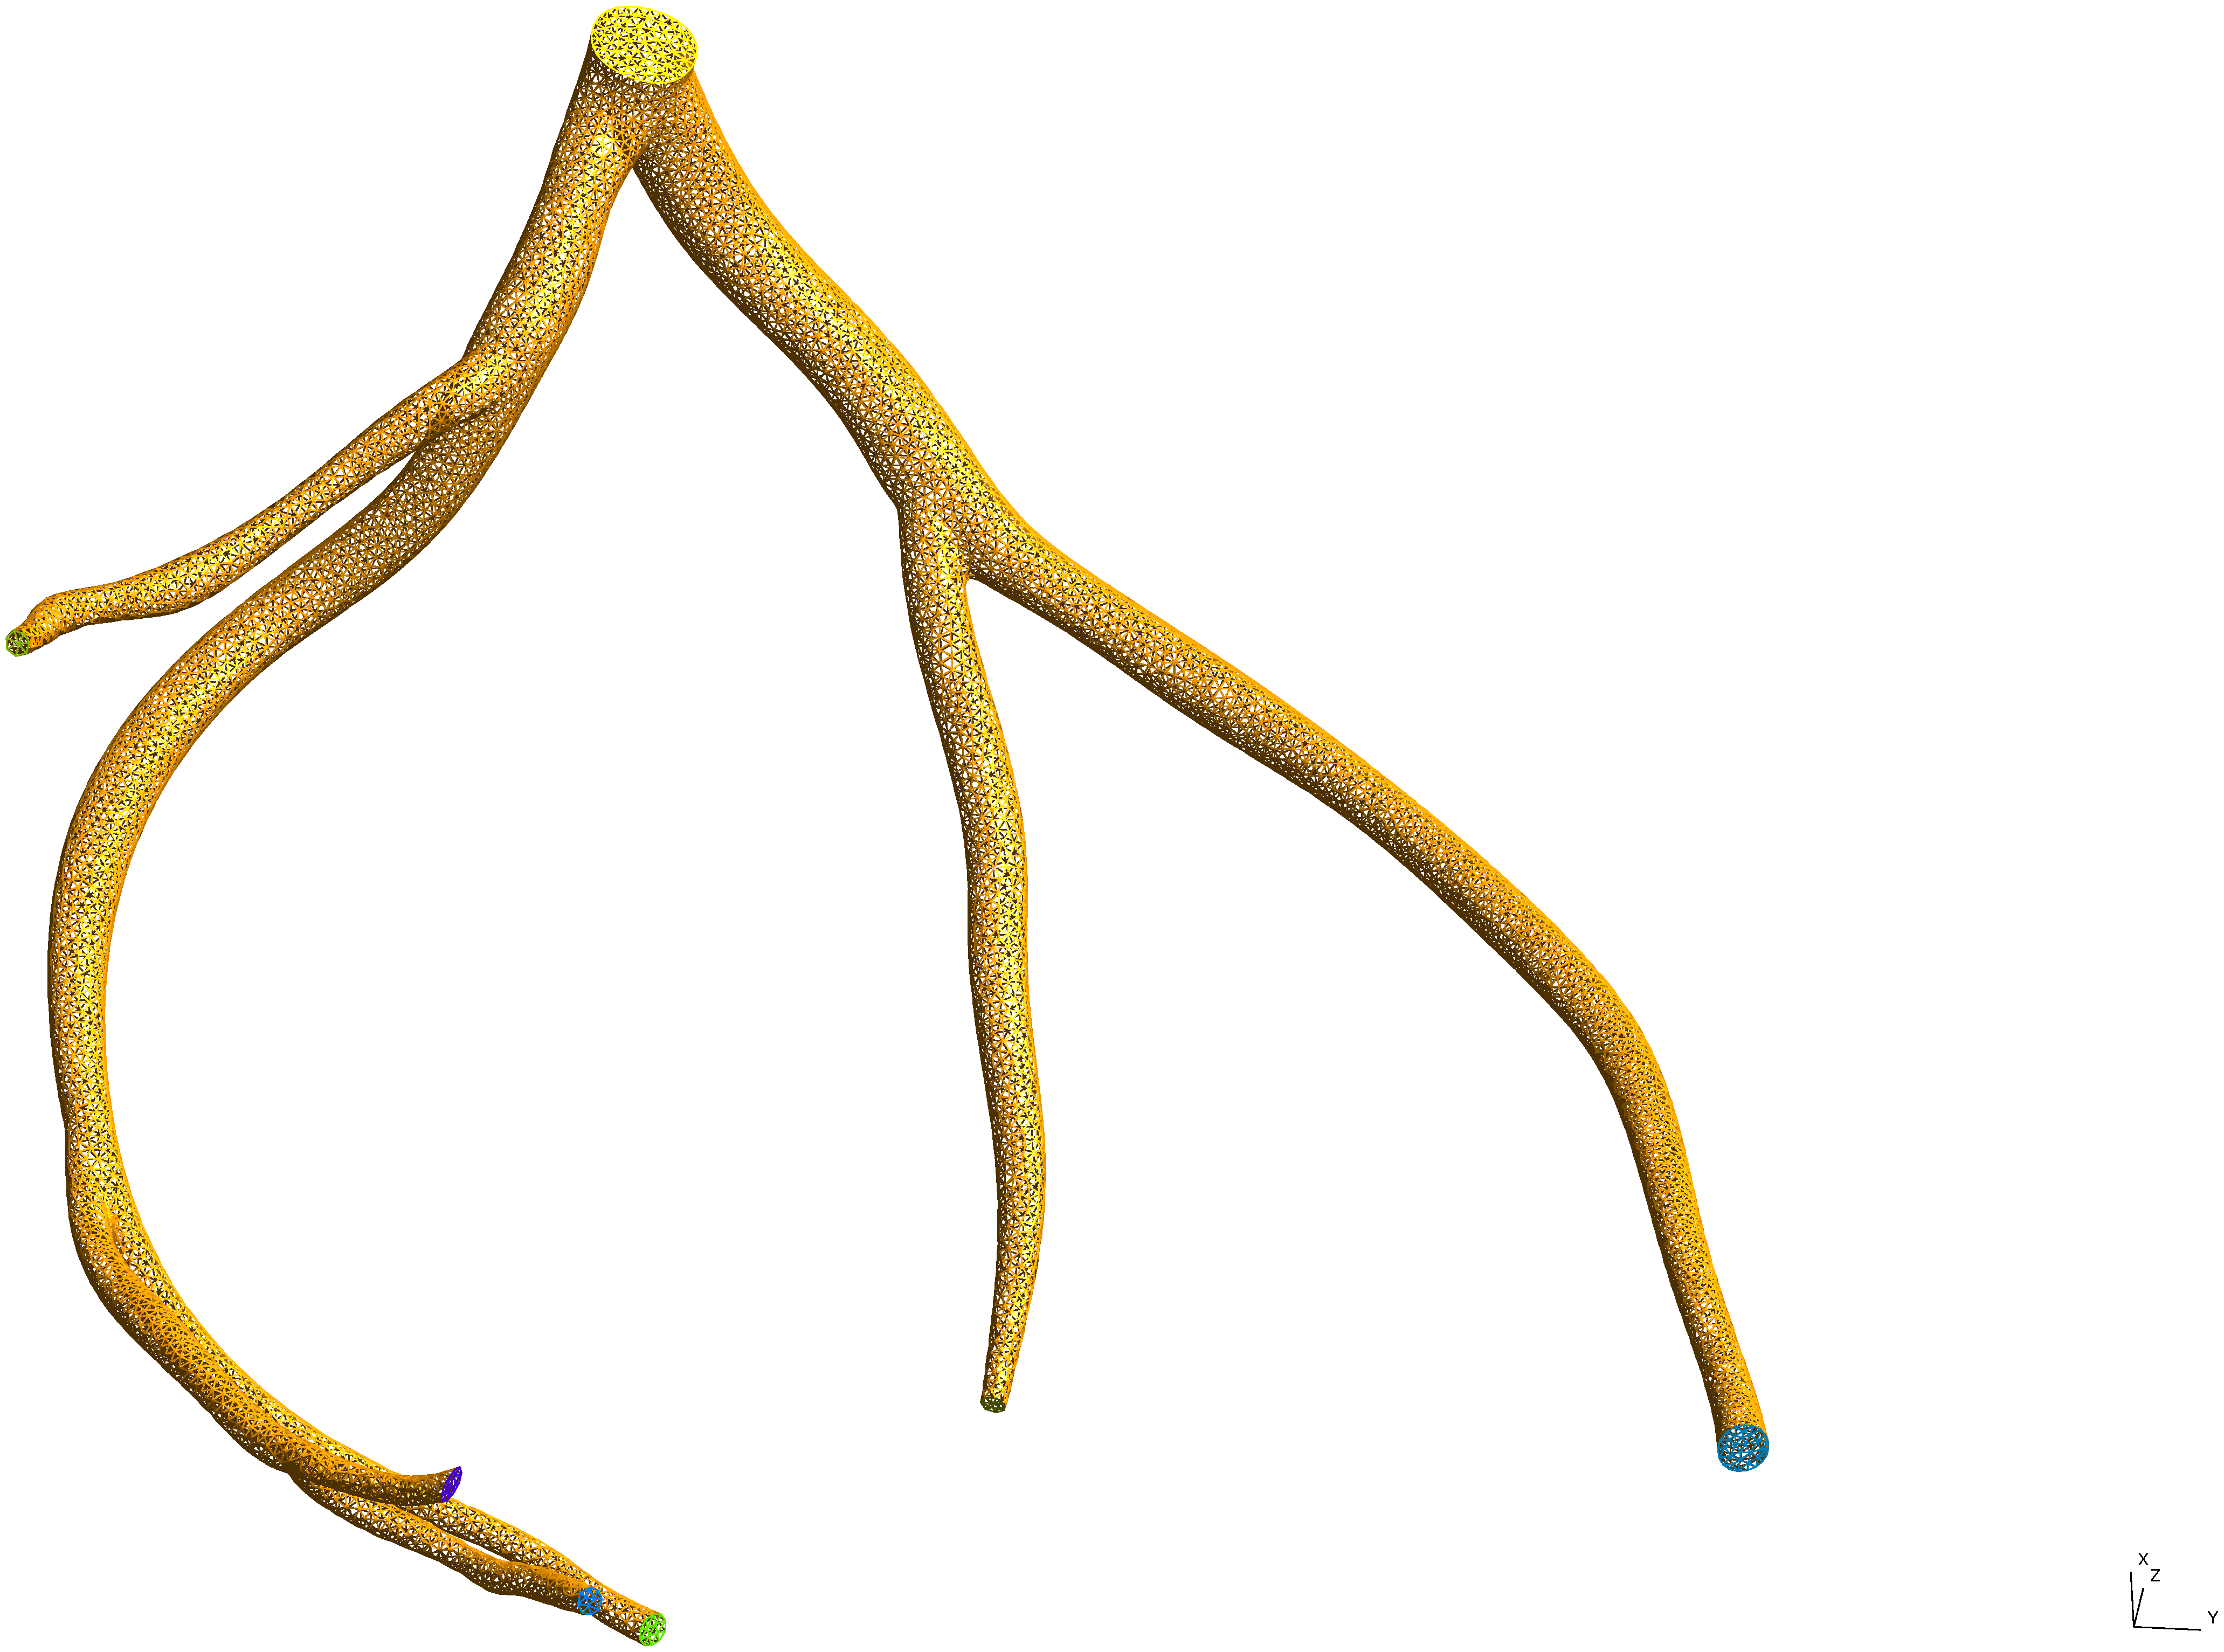
\includegraphics[width=13cm]{mesh_cropped.pdf}};
% Cover the residual gmsh axes glyph in the lower-right of the render
\fill[white] (11.9,-0.25) rectangle (13.15,1.0);
% ------------------------------------------------------------- boundary labels
% Inlet (yellow disc), fraction (0.288, 0.981)
\coordinate (inlet) at (3.744,9.417);
\draw[lead] (inlet) -- ++(-1.0,0.45) node[blk, anchor=east, font=\scriptsize, align=left]
  (inletlab) {$\Gamma_{\mathrm{in}}$:\; $\bm\sigma\bm n=-p_{\mathrm{ar}}(t)\,\bm n$};
% Wall
\coordinate (wallpt) at (6.845,5.404);
\draw[lead] (wallpt) -- ++(0.85,0.70) node[tag, anchor=west]
  {$\Gamma_{\mathrm{w}}$:\; $\bm u=\bm 0$};
% ------------------------------------------------------------------ outlets
% (fractions estimated from the render; small dots + tags)
\coordinate (o1) at (0.080,5.900);   % upper-left tip
\coordinate (o2) at (2.619,0.956);   % lower-left purple
\coordinate (o3) at (3.429,0.268);   % lower-left blue
\coordinate (o4) at (3.799,0.101);   % lower-left green
\coordinate (o5) at (5.785,1.437);   % mid-bottom
\coordinate (o6) at (10.204,1.169);   % bottom-right
\foreach \o/\i/\dx/\dy/\anch in {
  o1/1/-0.45/-0.10/east,
  o2/2/-0.60/0.40/east,
  o3/3/-0.35/-0.60/east,
  o4/4/0.45/-0.35/west,
  o5/5/0.35/-0.55/west,
  o6/6/0.50/-0.35/west}{
  \fill (\o) circle (1.6pt);
  \draw[lead] (\o) -- ++(\dx,\dy)
    node[tag, anchor=\anch] (t\i) {$\Gamma_\mu^{(\i)}$--$\mathcal{R}_\mu$RCR};
}
% ------------------------------------------------------------------- LV block
\node[blk, align=center] (act) at (15.9,10.3) {\scriptsize activation $\sigma_0(t)$};
\node[blk, below=0.35 of act, align=center] (lv)
  {reduced LV model\\[-1pt]{\scriptsize Caruel \emph{et al.} (2014)}};
\node[blk, below=0.4 of lv, align=center] (wk)
  {systemic Windkessel\\[-1pt]{\scriptsize$\mathcal{R}_p,C_p,\mathcal{R}_d,C_d$}};
\draw[siglead] (act) -- (lv);
\draw[siglead] (lv) -- (wk) node[midway, right=1pt]{\scriptsize $Q_{\mathrm{ar}}$};
\draw[siglead] ([xshift=-0.6cm]lv.west) -- (lv.west) node[midway, above]{\scriptsize $p_{\mathrm{LA}}$};
% p_ar to inlet
\draw[siglead] (wk.west) .. controls (11.2,9.2) and (7.5,10.4) .. ($(inlet)+(0.25,0.12)$)
  node[pos=0.35, above]{\scriptsize $p_{\mathrm{ar}}(t)$};
% p_LV to the terminal compartments (external loading)
\draw[dashlead] (lv.south east) .. controls (18.6,7.2) and (18.8,5.6) .. (17.5,4.85)
  node[pos=0.55, right, align=left]{\scriptsize $p_{\mathrm{LV}}(t)$\\[-2pt]\scriptsize $p_{\mathrm{im}}=\alpha\,p_{\mathrm{LV}}$};
% ------------------------------------------------------------- terminal inset
\begin{scope}[shift={(13.6,1.0)}]
  \draw[rounded corners=3pt, fill=white] (-0.25,-1.05) rectangle (5.75,3.55);% box
  \node[anchor=north west, font=\scriptsize\itshape] at (-0.15,3.50)
    {terminal outlet $i=1,\dots,6$};
  % circuit
  \draw (0.1,2.6) node[circ]{} node[above=1pt]{\scriptsize $p_{\mathrm{out}}^{(i)}$}
    to[vR, l_=\scriptsize $\mathcal{R}_{\mu,p}^{(i)}(Q_i)$] (2.6,2.6)
    node[circ]{} node[above=1pt]{\scriptsize $p_c^{(i)}$}
    to[vR, l_=\scriptsize $\mathcal{R}_{\mu,d}^{(i)}$] (5.1,2.6)
    node[circ]{} node[above=1pt]{\scriptsize $p_w$};
  \draw[siglead] (-0.55,2.6) -- (0.05,2.6);
  \node at (-0.62,2.95) {\scriptsize $Q_i$};
  % compliance to p_im reference
  \draw (2.6,2.6) to[C, l=\scriptsize $C^{(i)}$] (2.6,0.9);
  \draw[line width=0.9pt] (2.25,0.9) -- (2.95,0.9);
  \node[below] at (2.6,0.85) {\scriptsize $p_{\mathrm{im}}(t)=\alpha\,p_{\mathrm{LV}}$};
  % waterfall drainage
  \draw[siglead] (5.1,2.6) -- (5.1,1.5) node[below]{\scriptsize $P_{\mathrm{RA}}$};
  \node[right] at (5.15,2.05) {\scriptsize $Q_d^{(i)}$};
  % annotations
  \node[align=left, anchor=west, font=\scriptsize] at (-0.15,-0.15)
    {WRMS closure: $\mathcal{R}_{\mu,\ell}=8\mu_{\mathrm{eff}}(\dot\gamma_{a,\ell})L_\ell/(\pi R_\ell^{4}N_\ell)$\\
     $p_w=\max\!\left(p_{\mathrm{im}},P_{\mathrm{RA}}\right)$ (waterfall)\\
     $p_{tm}^{(i)}=p_c^{(i)}-p_{\mathrm{im}}$,\quad
     $C^{(i)}\dot p_{tm}^{(i)}=Q_i-Q_d^{(i)}$};
\end{scope}
% leader from representative outlet to inset
\draw[dashlead] (t6.east) .. controls (12.6,0.4) .. (13.5,1.4);
\end{tikzpicture}
\end{document}
